\begin{name}
	{\tenchude}
	{TOÁN 12}
	{LỚP TOÁN THẦY PHÁT}
	{Thời gian: 90 phút - Không kể thời gian phát đề}
\end{name}
\TN
\Opensolutionfile{ans}[ans/ansDe3-TN1]
\begin{ex}%[EX-Ôn Tập TN 2025,  Đỗ Vũ Minh Thắng]%[2D4N1-1]
	Hàm số nào sau đây là một nguyên hàm của hàm số $f(x) = \sin x$?
	\choice
	{$F_{1}(x) = \sin x$}
	{$F_{2}(x) = -\sin x$}
	{$F_{3}(x) = \cos x$}
	{\True $F_{4}(x) = -\cos x$}
	\loigiai{
		Vì $(-\cos x)'=\sin x$ nên $F_{4}(x)$ là một nguyên hàm của hàm số $f(x)$.
	}
\end{ex}

\begin{ex}%[2D4N1-1]%[To 20 - Dot 17 - Chuong 4 - Bai 3 - CD - De 1 - TN]%[Nguyễn Hữu Duy]
	Nếu $F(x)$ là nguyên hàm của hàm số $f(x)$, thì tích phân của $f(x)$ trên đoạn $[a;b]$ được tính như thế nào?
	\choice
	{\True $F(b)-F(a)$}
	{$F(a)-F(b)$}
	{$\dfrac{F(b)}{F(a)}$}
	{$\dfrac{F(a)}{F(b)}$}
	\loigiai
	{ Ta có
		$\displaystyle\int_{a}^{b} f(x) \mathrm{\,d}x = F(b) - F(a)$.
	}
\end{ex}

\begin{ex}%[2D4N1-2]
	Nguyên hàm của hàm số $f(x)=x^4+x^2$ là
	\choice
	{\True $\dfrac{1}{5}x^5+\dfrac{1}{3}x^3+C$}
	{$x^4+x^2+C$}
	{$x^5+x^3+C$}
	{$4x^3+2x+C$}
	\loigiai{
		$\displaystyle\int{f(x)\mathrm{\,d}x}=\displaystyle\int{(x^4+x^2)\mathrm{\,d}x}$ $=\dfrac{1}{5}x^5+\dfrac{1}{3}x^3+C$.}
\end{ex}

\begin{ex}%[2D4N1-3]%[Dự án EX-TF-TLN lần 3 -Mui Doan]
	Họ tất cả các nguyên hàm của hàm số $f(x)=\sin x$ là
	\choice
	{$-\sin x+C$}
	{$\cos x+C$}
	{$\dfrac{1}{2}\sin^2x+C$}
	{\True $-\cos x+C$}
	\loigiai{
		Ta có $\displaystyle\int f(x)\mathrm{\,d}x=\displaystyle\int\sin x\mathrm{\,d}x=-\cos x+C$.}
\end{ex}

\begin{ex}%[2D4N1-4]
	Hàm số nào dưới đây là một nguyên hàm của hàm số $f(x)=\sqrt{x}-1$ trên $(0;+\infty)$?
	\choice
	{$F(x)=\dfrac{1}{2\sqrt{x}}$}
	{$F(x)=\dfrac{1}{2\sqrt{x}}-x$}
	{$F(x)=\dfrac{2}{3}\sqrt[3]{x^2}-x+1$}
	{\True $F(x)=\dfrac{2}{3}\sqrt{x^3}-x+2$}
	\loigiai{
		Ta có : $\displaystyle\int (\sqrt{x}-1)\mathrm{d}x=\frac{2}{3}\sqrt{x^3}-x+C$.}
\end{ex}

\begin{ex}%[Mức độ 1]%[BG-12-New-4in1, Phạm Đức Thiệu]%[2D4N1-4]
	Tìm họ nguyên hàm của hàm số $f(x)=2^x$.
	\choice
	{$\displaystyle\int f(x)\mathrm{\,d}x=2^x+C$}
	{\True $\displaystyle\int f(x)\mathrm{\,d}x=\dfrac{2^x}{\ln 2}+C$}
	{$\displaystyle\int f(x)\mathrm{\,d}x=2^x\ln 2+C$}
	{$\displaystyle\int f(x)\mathrm{\,d}x=\dfrac{2^{x+1}}{x+1}+C$}
	\loigiai{
		Ta có $\displaystyle\int f(x)\mathrm{\,d}x=\displaystyle\int 2^x\mathrm{\,d}x=\dfrac{2^x}{\ln 2}+C$.
	}
\end{ex}

\begin{ex}%[2D4H1-2]
	Khẳng định nào sau đây \textbf{đúng}?
	\choice
	{\True $\displaystyle\int{\left( x-\dfrac{1}{x} \right)^2\mathrm{d}x} =\dfrac{x^3}{3}-2x-\dfrac{1}{x}+C$ }
	{ $\displaystyle\int{\left( x-\dfrac{1}{x} \right)^2\mathrm{d}x}=\dfrac{x^3}{3}-2x+\dfrac{1}{x}+C$ }
	{ $\displaystyle\int{\left( x-\dfrac{1}{x} \right)^2\mathrm{d}x} =\dfrac{1}{3}\left( x-\dfrac{1}{x} \right)^3+C$ }
	{ $\displaystyle\int{\left( x-\dfrac{1}{x} \right)^2\mathrm{d}x}=\dfrac{1}{3}\left( x-\dfrac{1}{x} \right)^3\left( 1+\dfrac{1}{x^2} \right)+C$ }
	\loigiai{
		Ta có $\displaystyle\int{\left( x-\dfrac{1}{x} \right)^2\mathrm{d}x}=\int{\left( x^2-2+\dfrac{1}{x^2} \right)\mathrm{d}x}=\dfrac{x^3}{3}-2x-\dfrac{1}{x}+C$.
	}
\end{ex}

\begin{ex}%[2D4H1-3]
	Tìm nguyên hàm của hàm số $f(x)=\sin x +6x$ là
	\choice
	{\True $-\cos x+3x^{2}+C$}
	{$\cos x +6x^{2}+C$}
	{$\cos x +C$}
	{$\cos x +3x^{2}+C$}
	\loigiai{ Ta có $\displaystyle\int\limits (\sin x +6x)\mathrm{\,d}x=-\cos x+3x^{2}+C$.
	}
\end{ex}

\begin{ex}%[Dự án 2025 - đề cấu trúc mới, Nguyễn Kiều Nhã Tú]%[2D4N2-1]
	Cho hàm số $y=f(x)$ liên tục trên đoạn $[a;b]$. Mệnh đề nào dưới đây là \textbf{sai}?
	\choice
	{$\displaystyle\int\limits_a^b f(x)\mathrm{\,d} x=-\displaystyle\int\limits_b^a f(x)\mathrm{\,d}x$}
	{\True $\displaystyle\int\limits_a^b f(x)\mathrm{\,d} x=\displaystyle\int\limits_a^c f(x)\mathrm{\,d} x+\displaystyle\int\limits_c^b f(x)\mathrm{\,d}x$, $\forall c \in \mathbb{R}$}
	{$\displaystyle\int\limits_a^b f(x)\mathrm{\,d} x=\displaystyle\int\limits_a^b f(t)\mathrm{\,d}t$}
	{$\displaystyle\int\limits_a^a f(x)\mathrm{\,d}x=0$}
	\loigiai{
		Theo tính chất của tích phân,  $\displaystyle\int\limits_a^b f(x) \mathrm{\,d}x=\displaystyle\int\limits_a^c f(x)\mathrm{\,d} x+\displaystyle\int\limits_c^b f(x) \mathrm{\,d}x$, $\forall c\in \mathbb{R}$ chỉ đúng khi $c\in[a;b]$.
	}
\end{ex}

\begin{ex}%[2D4N2-2]%[To 20 - Dot 17 - Chuong 4 - Bai 3 - CD - De 3]%[Đình Nguyên]
	Tích phân $\displaystyle\int\limits_{0}^{1}\left(2 x^{2}-1\right) \mathrm{\,d}x$ có giá trị bằng
	\choice
	{$1$}
	{$2$}
	{$\dfrac{1}{3}$}
	{\True $\dfrac{-1}{3}$}
	\loigiai
	{
	Ta có $ \displaystyle
		\int\limits_{0}^{1}\left(2 x^{2}-1\right) \mathrm{\,d}x=\left.\left(\dfrac{2 x^{3}}{3}-x\right)\right|_{0} ^{1}=\dfrac{-1}{3}
	$.
	}
\end{ex}

\begin{ex}%[2D4N2-3]
	Giá trị của $\displaystyle\int\limits_0^{\frac{\pi}{2}}{\sin x\mathrm{\,d}x}$ bằng
	\choice
	{0}
	{\True 1}
	{$-1$}
	{$\dfrac{\pi}{2}$}
	\loigiai{
	Tính được $\displaystyle\int\limits_0^{\frac{\pi}{2}}{\sin x\mathrm{\,d}x}=-\cos x\Big|_0^{\frac{\pi}{2}}=1$.}
\end{ex}

\begin{ex}%[Tổ 20 - Chương 4 - - CD]%[Nguyễn Văn Sang]%[2D4N2-4]
	Biết $I=\displaystyle\int\limits_0^1 3^x \cdot 7^{x+1} \cdot \mathrm{\,d} x=\dfrac{a}{\ln b+\ln c}$, trong đó $a, b, c \in \mathbb{Z}$ và $b, c$ là số nguyên tố.  Khi đó $a+b+c$ bằng
	\choice
	{\True $150$}
	{$147$}
	{$157$}
	{$140$}
	\loigiai{
		Ta có \[
			I=\displaystyle\int\limits_0^1 3^x \cdot 7^{x+1} \cdot \mathrm{\,d} x=7 \cdot \displaystyle\int\limits_0^1 21^x \cdot \mathrm{\,d} x=7 \cdot \dfrac{21^x}{\ln 21}\bigg|_0 ^1=\dfrac{140}{\ln 21}=\dfrac{140}{\ln 3+\ln 7}.
		\]
		Suy ra $a=140$, $b=3$, $c=7$ và $a+b+c=150$.
	}
\end{ex}
\Closesolutionfile{ans}

\TNTF
\Opensolutionfile{ans}[ans/ansDe3-TN2]
\begin{ex}%[2D4H1-1]%[Đào Trung Kiên]
	Xét hàm số $f(x)=\left(ax+b\right)^n$ với $a\neq 0$, $n \in \mathbb{R}\setminus \{0,1\}$ thì
	\choiceTF{\True $\displaystyle\int f(x)\mathrm{\,d}x=\dfrac{1}{a(n+1)}(ax+b)^{n+1}+C$}
	{$f'(x)=\dfrac{1}{a(n+1)}(ax+b)^{n+1}+C$}
	{\True Nếu $F(x)$ là một nguyên hàm của $f(x)$ và thỏa mãn $F\left(-\dfrac{b}{a}\right)=0$ thì $F(0)=\dfrac{b^{n+1}}{a(n+1)}$}
	{$\displaystyle\int f(x)\mathrm{\,d}x=\dfrac{1}{(n+1)}(ax+b)^{n+1}+C$}
	\loigiai{Với $f(x)=\left(ax+b\right)^n$ với $a\neq 0$, $n \in \mathbb{R}\setminus \{0,1\}$ thì ta có
		\begin{itemchoice}
			\itemch $\displaystyle\int f(x)\mathrm{\,d}x=\dfrac{1}{a(n+1)}(ax+b)^{n+1}+C$.
			\itemch Ta có $f'(x)=n(ax+b)^{n-1}$ nên khẳng định trong đề bài là sai.
			\itemch Nếu $F(x)$ là một nguyên hàm của $f(x)$ suy ra $F(x)=\dfrac{1}{a(n+1)}(ax+b)^{n+1}+C$ và thỏa mãn $F\left(-\dfrac{b}{a}\right)=0$ thì $C=0$ nên $F(0)=\dfrac{b^{n+1}}{a(n+1)}$.
			\itemch $\displaystyle\int f(x)\mathrm{\,d}x=\dfrac{1}{a(n+1)}(ax+b)^{n+1}+C$ là đúng nên $\displaystyle\int f(x)\mathrm{\,d}x=\dfrac{1}{(n+1)}(ax+b)^{n+1}+C$ là sai.
		\end{itemchoice}

	}
\end{ex}

\begin{ex}%[2D4H2-2]%[Tổ 20 - Đợt 17 - Chương 4 - - CD - Đề 7]%[Bình]
	Xét tính đúng sai của các mệnh đề sau:
	\choiceTF
	{\True $\displaystyle\int\limits_1^2 \dfrac{1}{x}\mathrm{\,d}x=\ln 2$}
	{\True $\displaystyle\int\limits_0^a \left(\dfrac{1}{\cos^2 x}+3\right)\mathrm{\,d}x=\tan a+3a$}
	{$\displaystyle\int\limits_m^n \dfrac{1}{x\sqrt{x}}\mathrm{\,d}x=2\left(\sqrt{m}-\sqrt{n}\right)$}
	{Có $2$ giá trị $a$ để $\displaystyle\int\limits_1^a 3x(x-2)\mathrm{\,d}x=0$}
	\loigiai
	{
		\begin{itemchoice}
			\itemch Đúng. $\displaystyle\int\limits_1^2 \dfrac{1}{x}\mathrm{\,d}x=\ln |x|\bigg\rvert_1^2=\ln 2$.
			\itemch Đúng. $\displaystyle\int\limits_0^a \left(\dfrac{1}{\cos^2 x}+3\right)\mathrm{\,d}x=(\tan x+3x)\bigg\rvert_0^a=\tan a+3a$.
			\itemch Sai. $\displaystyle\int\limits_m^n \dfrac{1}{x\sqrt{x}}\mathrm{\,d}x=\displaystyle\int\limits_m^n x^{\tfrac{-3}{2}}\mathrm{\,d}x=\dfrac{-2}{\sqrt{x}}\bigg\rvert_m^n=-2\left(\dfrac{1}{\sqrt{n}}-\dfrac{1}{\sqrt{m}}\right)$.
			\itemch Sai.
			\begin{eqnarray*}
				\displaystyle\int\limits_1^a 3x(x-2)\mathrm{\,d}x=\displaystyle\int\limits_1^a \left(3x^2-6x\right)\mathrm{\,d}x=\left(x^3-3x^2\right)\bigg\rvert_1^a&=&a^3-3a^2+2=0\\
				&\Leftrightarrow&\hoac{&a=1+\sqrt{3}\\&a=1-\sqrt{3}\\&a=1.}
			\end{eqnarray*}
			Vậy có $3$ giá trị $a$ để $\displaystyle\int\limits_1^a 3x(x-2)\mathrm{\,d}x=0$.
		\end{itemchoice}
	}
\end{ex}
\Closesolutionfile{ans}

\TNSA
\Opensolutionfile{ans}[ans/ansDe3-TN3]
\begin{ex}%[2D4H1-1]%[Đào Trung Kiên]
	Cho $F(x)$ là một nguyên hàm của hàm số $f(x) = ax + \dfrac{b}{x^2}$ $(x \neq 0)$. Biết $F(-1) = 1$, $F(1) = 4$, $f(1) = 0$. Tính giá trị của $M = 2a - b$ (làm tròn tới hàng phần mười).
	\shortans[]{$4,5$}
	\loigiai{
	Ta có $\displaystyle\int f(x)\mathrm{\,d}x = \displaystyle\int \left(ax + \dfrac{b}{x^2}\right)\mathrm{\,d}x = \dfrac{ax^2}{2} - \dfrac{b}{x} + C$.\\
	Theo giả thiết, ta có hệ phương trình $\heva{&F(-1) = 1 \\ &F(1) = 4 \\ &f(1) = 0} \Leftrightarrow \heva{&a + b + C = 1 \\ &a - b + C = 4 \\ &a + b = 0} \Rightarrow \heva{&a = \dfrac{3}{2} \\ &b = -\dfrac{3}{2}\cdot}$\\
	Vậy $M = 2a - b = 3 + \dfrac{3}{2} = \dfrac{9}{2}=4{,}5$
	}
\end{ex}

\begin{ex}%[2D4H2-2]%[Tổ 20 - Đợt 17 - Chương 4 - - CD - Đề 7]%[Lê Thị Thanh Tuyền]
	Cho hàm số $f(x)=a x^2+b x+c$ thỏa mãn $\displaystyle\int\limits_0^1f(x) \mathrm{\,d}x=28, \displaystyle\int\limits_{-1}^1f(x) \mathrm{\,d} x=52$ và $\displaystyle\int\limits_0^2f(x) \mathrm{\,d} x=66$. Giá trị của biểu thức $P=a^b. c$ là
	\shortans{$2025$}

	\loigiai{
		\begin{itemize}
			\item Ta có: $\displaystyle\int f(x) \mathrm{\,d} x=\displaystyle\int\left(a x^2+b x+c\right) d x=\dfrac{a}{3} x^3+\dfrac{b}{2} x^2+c x+C$.
			\item  $\displaystyle\int\limits_0^1f(x)\mathrm{\,d} x=\left.28\Rightarrow\left(\dfrac{a}{3} x^3+\dfrac{b}{2} x^2+c x\right)\right|_0 ^1=28\Leftrightarrow \dfrac{1}{3} a+\dfrac{1}{2} b+c=28 \quad (1)$.
			\item 	$\displaystyle\int\limits_{-1}^1f(x) \mathrm{\,d} x=\left.52\Rightarrow\left(\dfrac{a}{3} x^3+\dfrac{b}{2} x^2+c x\right)\right|_{-1} ^1=52\Leftrightarrow \dfrac{2}{3} a+2c=52 \quad (2)$.
			\item 	$\displaystyle\int\limits_0^2f(x)\mathrm{\,d} x=\left.66\Rightarrow\left(\dfrac{a}{3} x^3+\dfrac{b}{2} x^2+c x\right)\right|_0 ^2=66\Leftrightarrow \dfrac{8}{3} a+2b+2c=66 \quad (3)$.
			\item 	Từ $(1), (2)$ và $(3)$ ta có hệ phương trình: $\heva{&\dfrac{1}{3} a+\dfrac{1}{2} b+c=28\\& \dfrac{2}{3} a+2c=52\\& \dfrac{8}{3} a+2b+2c=66}\Leftrightarrow\heva{&a=3\\&b=4\\&c=25.}$
			\item Vậy $P=3^4.25=2025$.
		\end{itemize}
	}
\end{ex}

\begin{ex}%[2D4H3-1]%[Tổ 21 - Đợt 17 - Chương 4 - - Cánh Diều - Đề 2]
	Cho hàm số $f(x)=\heva{&7-4 x^{3} \text { khi } 0 \leq x \leq 1 \\ &4-x^{2} \text { khi } x>1}$. Tính diện tích hình phẳng giới hạn bởi đồ thị hàm số $f(x)$ và các đường thẳng $x=0$, $x=3$, $y=0$.
	\shortans{$10$}
	\loigiai
	{\immini{Ta có
			\begin{align*}
				S & =\displaystyle\int_{0}^{1} (7-4 x^{3}) \mathrm{d}x+\displaystyle\int_{1}^{2} (4-x^{2}) \mathrm{d}x+\displaystyle\int_{2}^{3}( x^{2}-4) \mathrm{d}x \\
				  & =7 x-\left.x^{4}\right|_{0} ^{1}+\left.\left(4 x-\dfrac{x^{3}}{3}\right)\right|_{1} ^{2}+\left.\left(\dfrac{x^{3}}{3}-4 x\right)\right|_{2} ^{3}   \\
				  & =6+4-\dfrac{7}{3}-3-\dfrac{8}{3}+8=10.
			\end{align*}}{
			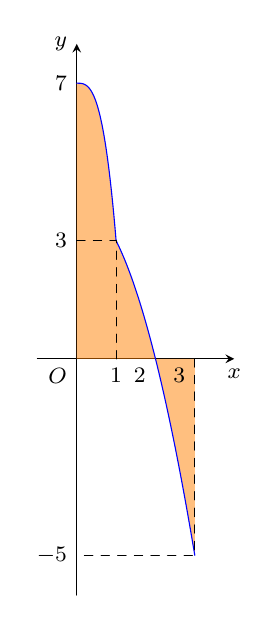
\begin{tikzpicture}[scale=.5,font=\footnotesize, line join=round,line cap=round,>=stealth]
				\draw[->] (-1,0)--(4,0) node[below] {$x$};
				\draw[->] (0,-6)--(0,8) node[left] {$y$};
				% Tô vùng giữa x=2 và x=3, trục Ox và đồ thị 4-x^2
				\fill[fill=orange, opacity=0.5]
				(2,0) -- plot[domain=2:3, samples=100] (\x,{4-(\x)^2}) -- (3,0) -- cycle;
				\fill[fill=orange, opacity=0.5]
				(1,0) -- plot[domain=1:2, samples=100] (\x,{4-(\x)^2}) -- (2,0) -- cycle;
				\fill[fill=orange, opacity=0.5]
				(0,0) -- plot[domain=0:1, samples=100] (\x,{7-4*(\x)^3}) -- (1,0) -- cycle;
				% Vẽ các đồ thị hàm số
				\draw[color=blue, samples=100, domain=0:1] plot(\x,{7-4*(\x)^3});
				\draw[color=blue, samples=100, domain=1:3] plot(\x,{4-(\x)^2});
				% Đường nét đứt và chú thích các điểm
				\draw[dashed] (0,3)--(1,3)--(1,0) (3,0)--(3,-5)--(0,-5);
				\node[left] at (0,3) {$3$};
				\node[left] at (0,7) {$7$};
				\node[left] at (0,-5) {$-5$};
				\node[below left] at (0,0) {$O$};
				\node[below] at (1,0) {$1$};
				\node[below left] at (2,0) {$2$};
				\node[below left] at (3,0) {$3$};
			\end{tikzpicture}
		}
	}
\end{ex}

\begin{ex}%[Nguyễn Tuấn, dự án sáng tác đề 12]%[2D4H3-3]
	\immini
	{
		Một vật trang trí có dạng khối tròn xoay tạo thành khi quay miền $(R)$ được giới hạn bởi đường gấp khúc $DABFE$ và cung tròn $ED$ (phần gạch chéo trong hình bên) xung quanh trục $AB$. Biết $ABCD$ là hình chữ nhật cạnh $AB =3$ cm, $AD=2$ cm; $F$ là trung điểm của $BC$; điểm $E$ cách $AD$ một đoạn bằng $1$ cm. Tính thể tích của vật trang trí đó, làm tròn kết quả đến hàng phần mười, đơn vị cm$^3$.
		\shortans{$16{,}5$}
	}
	{
		\begin{tikzpicture}[scale=1.2, line join=round, line cap=round,>=stealth,font=\footnotesize]
			\path (0,0) coordinate (B)	(2,0) coordinate (C) (2,3) coordinate (D) (0,3) coordinate (A) ($(B)!.5!(C)$) coordinate (F) ($(F)+(0,2)$) coordinate (E) ($(A)!.5!(D)$) coordinate (I) ;
			\draw (A)--(B)--(C)--(D)--cycle (E)--(F);
			\draw[dashed] (E)--(I);
			\foreach \d/\g in {A/90,B/-90,C/0,D/90,F/-90,E/-60}
			\draw[fill=black] (\d) circle (1pt) +(\g:0.2) node{$\d$};
			\draw (E) arc (-90:0:1cm);
			\fill[color=gray,opacity=0.5] (A)--(B)--(F)--(I)--cycle (E) arc (-90:0:1cm)--(D)--(I)--cycle;
		\end{tikzpicture}
	}
	\loigiai{
		\immini
		{
			Gắn hệ trục tọa độ như hình vẽ bên.\\
			Quay hình chữ nhật $GEFB$ xung quanh trục $AB$ ta được khối trụ có bán kính đáy bằng $1$ và chiều cao bằng $2$.\\
			Phương trình đường tròn tâm $I$ bán kính bằng $1$ là $x^2+(y-1)^2=1$, suy ra phương trình của cung $DE$ là $y=1+\sqrt{1-x^2}$.\\
			Vây thể tích của vật trang trí là
			\[V=\pi \displaystyle\int\limits_{0}^{1} \left(1+\sqrt{1-x^2}\right)^2 \mathrm{\,d}x+\pi \cdot 1^2\cdot 2\approx 16{,}5\ (\mathrm{cm}^3).\]
		}
		{
			\begin{tikzpicture}[scale=1.2, line join=round, line cap=round,>=stealth,font=\footnotesize]
				\draw[->] (-0.5,0)--(4,0) node[below]{$x$};
				\draw[->] (0,-0.5)--(0,3) node[left]{$y$};
				\path (0,0) coordinate (A)	(3,0) coordinate (B) (3,2) coordinate (C) (0,2) coordinate (D) ($(B)!.5!(C)$) coordinate (F) ($(F)-(2,0)$) coordinate (E) ($(A)!.5!(D)$) coordinate (I) (1,0) coordinate (G) ;
				\draw (A)--(B)--(C)--(D)--cycle (E)--(F);
				\draw[dashed] (E)--(I) (E)--(G);
				\foreach \d/\g in {A/-120,B/-90,C/0,D/120,F/0,E/-60,I/180,G/-90}
				\draw[fill=black] (\d) circle (1pt) +(\g:0.2) node{$\d$};
				\draw (E) arc (0:90:1cm);
				\fill[color=gray,opacity=0.5] (A)--(B)--(F)--(I)--cycle (E) arc (0:90:1cm)--(D)--(I)--cycle;
			\end{tikzpicture}
		}
	}
\end{ex}

\Closesolutionfile{ans}

\TNTF
\begin{ex}%[2D4H2-2]
	Tính tích phân $A=\displaystyle\int\limits_{-3}^5 {\left(|x+2|-|x-2|\right)}\mathrm{\,d}x$.

	\loigiai{
	$A=\displaystyle\int\limits_{-3}^5 {\left(|x+2|-|x-2|\right)}\mathrm{\,d}x$.\\
	Ta có bảng xét dấu để phá trị tuyệt đối:
	\begin{center}
		
\begin{tikzpicture}
			\tkzTabInit[nocadre=false,lgt=3,espcl=2.5,deltacl=0.5]
			{$x$/.6,$|x+2|$/.6,$|x-2|$/.6,$|x+2|+|x-2|$/.6}
			{$-3$,$-2$,$2$,$5$}
			\tkzTabLine{,-x-2,0,x+2,|,-x-2,}
			\tkzTabLine{,-x+2,|,-x+2,0,x-2,}
			\tkzTabLine{,-4,|,2x,|,4,}
		\end{tikzpicture}
	\end{center}
	Khi đó
	\begin{eqnarray*}
		A=	\displaystyle\int\limits_{-3}^5 {\left(|x+2|-|x-2|\right)}\mathrm{\,d}x
		&=& \displaystyle\int\limits_{-3}^{-2} {(-4)}\mathrm{\,d}x +
		\displaystyle\int\limits_{-2}^2 {2x}\mathrm{\,d}x +
		\displaystyle\int\limits_2^5 {4}\mathrm{\,d}x\\
		&=& -4x \Big|_{-3}^{-2} + x^2 \Big|_{-2}^2 + \cdot 4x \Big|_2^5=8.
	\end{eqnarray*}
	}
\end{ex}


\begin{ex}%[2D4V1-4]
	Cho hàm số $ y=f(x)$ đồng biến và có đạo hàm liên tục trên $\mathbb{R}$ thỏa mãn $\left(f'(x)\right)^2=f(x)\cdot\mathrm{e}^x$, $\forall x\in\mathbb{R}$ và $f(0)=2$. Tính $ f(2)$. (Kết quả làm tròn đến hàng phần trăm).
	% \shortans{$9{,}81$}
	\loigiai{
	Vì hàm số $ y=f(x)$ đồng biến và có đạo hàm liên tục trên $\mathbb{R}$ đồng thời $ f(0)=2$ nên $f'(x)\ge 0$ và $ f(x)>0$ với mọi $ x\in\left[0;+\infty\right)$.\\
	Từ giả thiết $\left(f'(x)\right)^2=f(x)\cdot \mathrm{e}^x$, $\forall x\in\mathbb{R}$ suy ra $f'(x)=\sqrt{f(x)}\cdot\mathrm{e}^{\tfrac{x}{2}}$, $\forall x\in\left[0;+\infty\right).$\\
	Do đó $\dfrac{f'(x)}{2\sqrt{f(x)}}=\dfrac{1}{2}{\mathrm{e}^{\tfrac{x}{2}}}$, $\forall x\in\left[0;+\infty\right).$\\
	Lấy nguyên hàm hai vế, ta được $\sqrt{f(x)}=e^{\tfrac{x}{2}}+C$, $\forall x\in\left[0;+\infty\right)$ với $C$ là hằng số.\\
	Kết hợp với $ f(0)=2$, ta được $C=\sqrt{2}-1$.\\
	Suy ra $ f(2)=\left(\mathrm{e}+\sqrt{2}-1\right)^2\approx 9{,}81$.}
\end{ex}

\begin{ex}%[EX-Ôn Tập TN 2025, Võ Thanh Phong]%[2D4C3-2]
	Một cổng có đạng hình parabol với chiều cao $8$ m, chiều rộng chân đế $8$ m. Người ta căng hai sợi dây trang trí $AB$,  $CD$ nằm ngang, đồng thời chia cổng thành ba phần sao cho hai phần ở phía trên có diện tích bằng nhau. Tỉ số $\dfrac{CD}{AB}$ bằng bao nhiêu (làm tròn kết quả đến hàng phần trăm)?
	\begin{center}
		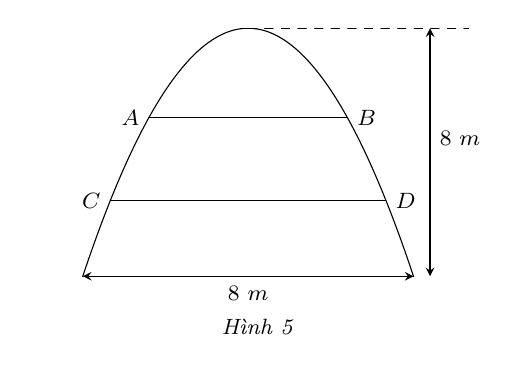
\begin{tikzpicture}[scale=0.7, font=\footnotesize, line join=round, line cap=round,>=stealth]
			\begin{scope}
				\clip (-4,-4.5) rectangle (4,0);
				\draw [smooth,domain=-5:4, samples=200] plot (\x, {-0.5*(\x)^2});
			\end{scope}
			\draw [<->] (3.3,0)--(3.3,-4.5);
			\node[right] at (3.3,-2){$8\,\,m$};
			\draw [<->] (-3,-4.5)--(3,-4.5);
			\node[below] at (0,-4.5){$8\,\,m$};
			\node[left] at (-1.8,-1.62){$A$};
			\node[right] at (1.8,-1.62){$B$};
			\node[left] at (-2.5,-3.125){$C$};
			\node[right] at (2.5,0-3.125){$D$};
			\draw [-] (-1.8,-1.62)--(1.8,-1.62);
			\draw [-] (-2.5,-3.125)--(2.5,0-3.125);
			\draw [dashed] (0,0)--(4,0);
			\node[below] at (current bounding box.south){\textit{Hình 5}};
		\end{tikzpicture}
	\end{center}
	% \shortans{ $1{,}26$}
	\loigiai{
	\immini{Gắn hệ trục tọa độ $Oxy$ vào cổng parabol như hình bên với trục $Oy$ trùng với đường đối xứng của parabol, gốc $O$ nằm ở đỉnh của parabol, đơn vị trên mỗi trục tính theo mét. Khi đó, phương trình parabol có dạng $y=ax^2$.\\
		Vì parabol đi qua điểm có toạ độ $(-4 ;-8)$ nên $a=-\dfrac{1}{2}$. Suy ra phương trình parabol là $y=-\dfrac{1}{2} x^2$.\\}{
		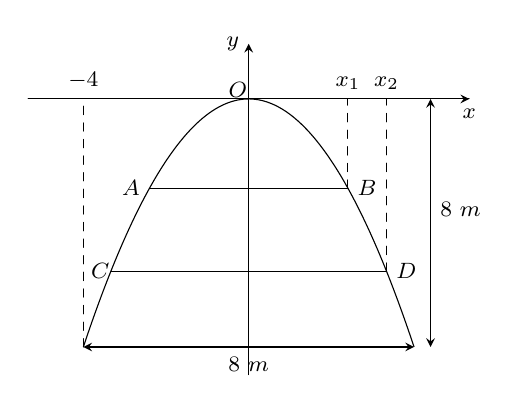
\begin{tikzpicture}[scale=0.7, font=\footnotesize, line join=round, line cap=round,>=stealth]
			\draw[->] (-4,0) --(4,0) node[below]{$x$};
			\draw[->] (0,-5) --(0,1) node[left]{$y$};
			\draw (0,0) node[above left=-3pt]{$O$};
			\begin{scope}
				\clip (-4,-4.5) rectangle (4,0);
				\draw [smooth,domain=-5:4, samples=200] plot (\x, {-0.5*(\x)^2});
			\end{scope}
			\draw [<->] (3.3,0)--(3.3,-4.5);
			\node[right] at (3.3,-2){$8\,\,m$};
			\draw [<->] (-3,-4.5)--(3,-4.5);
			\node[below] at (0,-4.5){$8\,\,m$};
			\node[left] at (-1.8,-1.62){$A$};
			\node[right] at (1.8,-1.62){$B$};
			\node[left=-3pt] at (-2.5,-3.125){$C$};
			\node[right] at (2.5,0-3.125){$D$};
			\draw [-] (-1.8,-1.62)--(1.8,-1.62);
			\draw [-] (-2.5,-3.125)--(2.5,0-3.125);
			\draw [dashed] (0,0)--(4,0) (1.8,-1.62)--(1.8,0) (2.5,0-3.125)--(2.5,0) (-3,-4.5)--(-3,0);
			\node[above] at (1.8,0){$x_1$};
			\node[above] at (2.5,0){$x_2$};
			\node[above] at (-3,0){$-4$};
		\end{tikzpicture}}
	Giả sử $B$ có hoành độ $x_1$,  $D$ có hoành độ $x_2$. Khi đó, phương trình đường thẳng $AB$ là $y=-\dfrac{1}{2} x_1^2$, phương trình đường thẳng $CD$ là $y=-\dfrac{1}{2} x_2^2$.\\
	Diện tích hình phẳng giới hạn bởi parabol và đường thẳng $AB$ là
	\[
		S_1=2\displaystyle\int\limits_0^{x_1}\left[-\dfrac 12x^2-\left(-\dfrac 12x_1^2\right)\right]\mathrm{\,d} x=\left.2\left(-\dfrac{x^3}6+\dfrac{x_1^2}2x\right)\right|_0^{x_1}=\dfrac 23x_1^3\,\,\left(\mathrm{m}^2\right).
	\]
	Diện tích hình phẳng giới hạn bởi parabol và đường thẳng $CD$ là
	\[
		S_2=2\displaystyle\int\limits_0^{x_2}\left[-\dfrac 12x^2-\left(-\dfrac 12x_2^2\right)\right]\mathrm{\,d} x=\left.2\left(-\dfrac{x^3}6+\dfrac{x_2^2}2x\right)\right|_0^{x_2}=\dfrac 23x_2^3\,\,\left(\mathrm{m}^2\right).
	\]
	Theo giả thiết, ta có  $S_2=2S_1\Leftrightarrow x_2^3=2x_1^3\Leftrightarrow\dfrac{x_2}{x_1}=\sqrt[3]2\approx 1{,}26$.\\
	Khi đó, $\dfrac{CD}{AB}=\dfrac{2x_2}{2x_1}\approx 1{,}26$.
	}
\end{ex}

% \Closesolutionfile{ansbook}
% \HetDe
% \label{De3}
% %
% \cleardoublepage
% \setcounter{page}{1}
% \rfoot{Trang \thepage/\pageref{DA3} - Đáp án trắc nghiệm Mã đề 3}
% \begin{center}
% 	\bfseries ĐÁP ÁN TRẮC NGHIỆM MÃ ĐỀ 3
% \end{center}

% \inputansbox{10}{ans/ansDe3-TN1}
% \inputansbox[3]{2}{ans/ansDe3-TN2}
% \inputansbox{3}{ans/ansDe3-TN3}
% \label{DA3}
%
